%% LyX 2.1.0 created this file.  For more info, see http://www.lyx.org/.
%% Do not edit unless you really know what you are doing.
\documentclass[oneside]{jsbook}
\usepackage[japanese]{babel}
\usepackage{url}
\usepackage{graphicx}

\makeatletter
%%%%%%%%%%%%%%%%%%%%%%%%%%%%%% User specified LaTeX commands.
\date{}
\usepackage{url}
\setlength{\textwidth}{\fullwidth}
\setlength{\evensidemargin}{\oddsidemargin}

\@ifundefined{showcaptionsetup}{}{%
 \PassOptionsToPackage{caption=false}{subfig}}
\usepackage{subfig}
\makeatother

\begin{document}

\title{VirtualBoxを用いた仮想マシンの構築}


\author{首都大学東京マイクロコンピュータ研究会\\
nosada}

\maketitle

\chapter{はじめに}


\section{この文書について}

VirtualBoxを用いた仮想マシンの構築(以下``この文書''と表記)は、「Arch Linuxインストールガイド」%
\footnote{この文書が入っているディレクトリの中にあるALIG.pdfが該当する。%
}に付随して、既存のOSをすり潰すこと無く新規にOSを試すために、Oracle VM VirtualBox%
\footnote{\url{https://www.virtualbox.org/}%
}を使用して仮想のコンピュータを構築する手順を説明するものです。


\section{前書き}

本来OSはコンピュータというハードウェアを動作させるために用いるものです。私達が普段使用しているパソコンにも、各々の用途、目的に最適化されたOSがすでに構築されていると思います。せっかく今まで時間を掛けて構築してきた環境をOSインストールの為に潰してしまおうと考える人はおそらく皆無でしょう%
\footnote{もちろん既存環境をぶっ潰してやるという気概を持つ方がいても何一つおかしくない。しかしそのような方が求める知識はこの文書では扱っていない。%
}。

そこで、既存の環境の上に仮想のコンピュータを構築する仮想化ソフトウェアを使用して、いくらでもいじくり回してぶっ壊しても構わないコンピュータを作成することにしましょう。

仮想化ソフトウェアにはOracle VM VirtualBox(以下VirtualBox)を使用します。

以下では、VirtualBoxのインストールは既に済んでいるものとして話を進めていきます。また、以下に説明のために用いた画像はKDE
4.10%
\footnote{X window systemを使用するOSにおけるデスクトップ環境の一つ。筆者が好んで使っている。\url{http://www.kde.org/}%
}上のものですので、WindowsやOS X等でのものとはUIが異なる場合があります。その場合は適当に推察をしてそれらしい感じのものを選択してください。

また、ここで構築するマシンを「仮想マシン」、VirtualBoxを動作させるマシンを「物理マシン」と呼称します。


\chapter{仮想マシンの構築}


\section{仮想マシンの生成}

適当な方法でVirtualBoxを起動すると、``Oracle VM VirtualBox マネージャー''(図\ref{OracleVMVBoxManager})というウィンドウが立ち上がると思います(図中では既にマシンが存在していますが通常初回起動時はは何もない状態です)。ここで「新規」をクリックすると図\ref{BuildVM_NameAndOS_Default}のようなウィンドウが新たに表示されます。ウィンドウ内のテキストボックスに適当な仮想マシンの名前を入力し、プルダウンメニューからOSの種類を選択します。今回はArch
Linux x86\_64(64ビット版)をインストールするので、図\ref{BuildVM_NameAndOS}のように選択します。設定後は以下のようになります。これ以降、作成したマシンを指定する必要がある際は、ここで設定したマシンの名前(Dicke\_Berta)を用います。仮想マシンの名前は任意に決めて頂いて構いません。``Dicke\_Berta''は一例です。
\begin{itemize}
\item 名前:任意
\item タイプ:Linux
\item バージョン:Arch Linux(64 bit)
\end{itemize}
設定後、「次へ」をクリックします。すると図\ref{BuildVM_MemSize}のウィンドウが現れます。

\begin{center}
\begin{figure}[!tbh]
\centering{}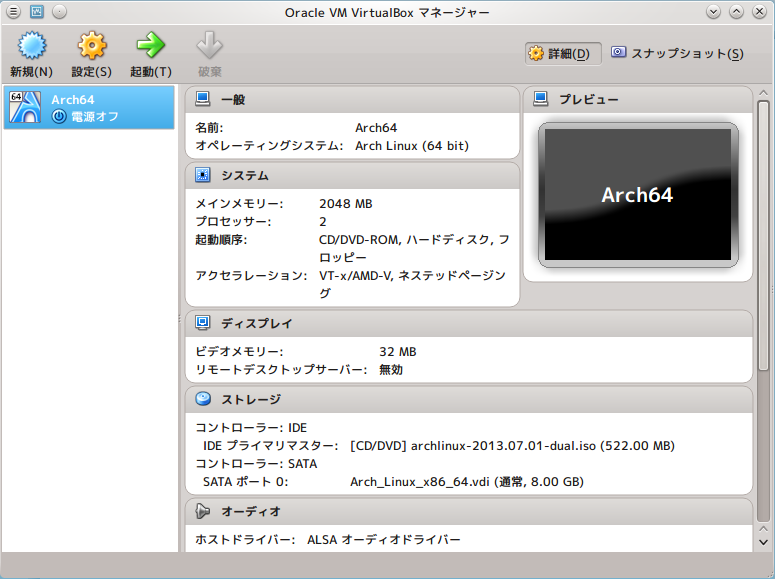
\includegraphics[scale=0.5]{Figs/Fig_VBox/OracleVMVBoxManager1}\protect\caption{Oracle VM VirtualBox マネージャー}
\label{OracleVMVBoxManager}
\end{figure}

\par\end{center}

\begin{center}
\begin{figure}[!tbh]
\centering{}\subfloat[デフォルト]{\begin{centering}
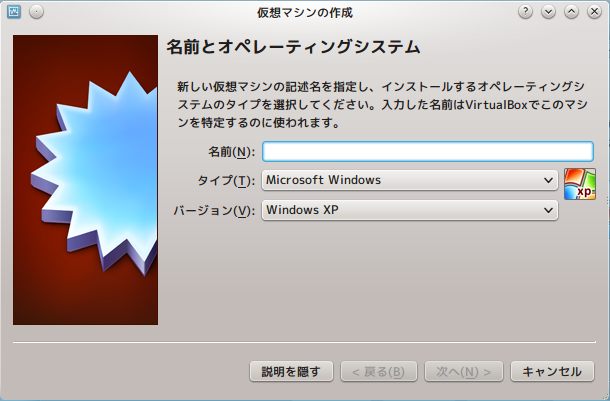
\includegraphics[scale=0.5]{Figs/Fig_VBox/BuildVM_NameAndOS1}
\par\end{centering}

\centering{}\label{BuildVM_NameAndOS_Default}}\\
\subfloat[設定後]{\centering{}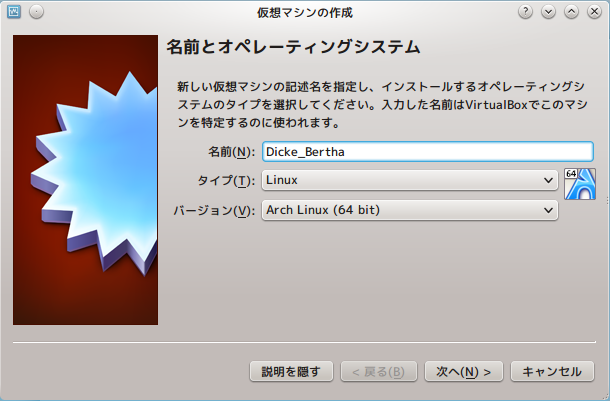
\includegraphics[scale=0.5]{Figs/Fig_VBox/BuildVM_NameAndOS2}\label{BuildVM_NameAndOS}}\protect\caption{仮想マシンの作成(コンピュータ名とOSの設定)}
\end{figure}

\par\end{center}

続いて、仮想マシンが使用するRAMのサイズを設定します。物理マシンに搭載されているRAMの量にもよりますが、おおよそ搭載メモリの$1/4$程度がよろしいでしょう。ここであまりに大量なメモリを設定すると物理マシン上の既存システムが不安定になります。また、ここで1GB未満のメモリを割り当てる設定をした場合、仮想マシン上で構築する環境によっては、不足するメモリ領域を仮想マシンが使用するディスク上の専用領域%
\footnote{これをスワップ領域という。%
}で補う必要が出てきます。この結果動作速度の低下が見込まれますので、1GB以上のメモリ領域を割り当てることを推奨します。

設定後、「次へ」をクリックし、図\ref{BuildVM_HardDrive}のウィンドウへ移ります。

\begin{figure}[!tbh]
\centering{}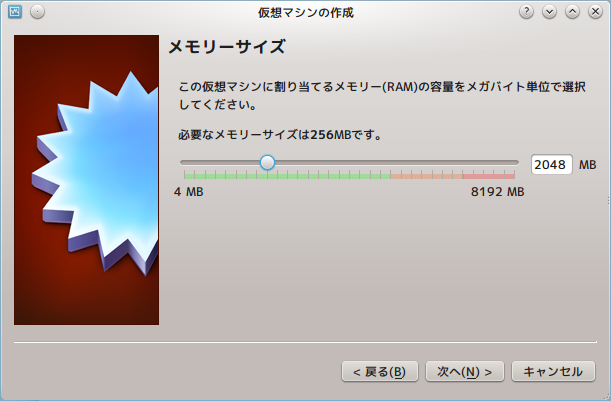
\includegraphics[scale=0.5]{Figs/Fig_VBox/BuildVM_MemSize}\protect\caption{仮想マシンの作成(RAMサイズの設定)}
\label{BuildVM_MemSize}
\end{figure}


次に仮想マシンが使用するディスク(以下``仮想ディスク'')を設定します。今回は新規に仮想マシンを作成し、仮想マシンに用いるための既存の仮想ディスク(ハードドライブ)が存在しない状態ですので、ラジオボタン中から「仮想ハードドライブを作成する」を選択し、「作成」をクリックします。すると図\ref{BuildVHD_TypeOfHardDrive}のウィンドウに遷移します。

\begin{figure}[!tbh]
\centering{}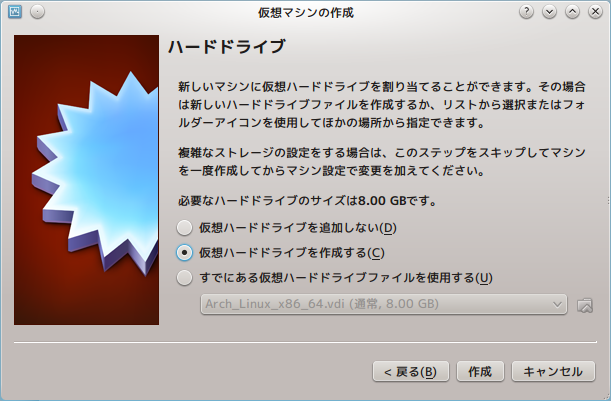
\includegraphics[scale=0.5]{Figs/Fig_VBox/BuildVM_HardDrive}\protect\caption{仮想マシンの作成(ディスクの設定)}
\label{BuildVM_HardDrive}
\end{figure}


図\ref{BuildVHD_TypeOfHardDrive}は仮想ディスクの形式を設定します。今回は仮想マシンをVirtualBox上のみでの運用としますので、画面の指示通り何もいじらず、デフォルトのVDI(VirtualBox
Disk Image)が選択されている状態で、「次へ」をクリックします。

\begin{figure}[!tbh]
\centering{}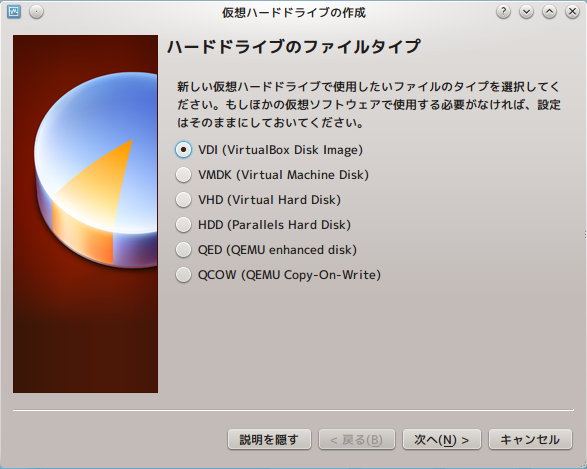
\includegraphics[scale=0.5]{Figs/Fig_VBox/BuildVHD_TypeOfHardDrive}\protect\caption{仮想ハードディスクの作成(ディスクタイプの設定)}
\label{BuildVHD_TypeOfHardDrive}
\end{figure}


続いて遷移する図\ref{BuildVHD_StorageOnVHD}は、仮想ディスクのサイズ確保の設定です。今回は「可変サイズ」を選択します。設定後、「次へ」をクリックします。

\begin{figure}[!tbh]
\centering{}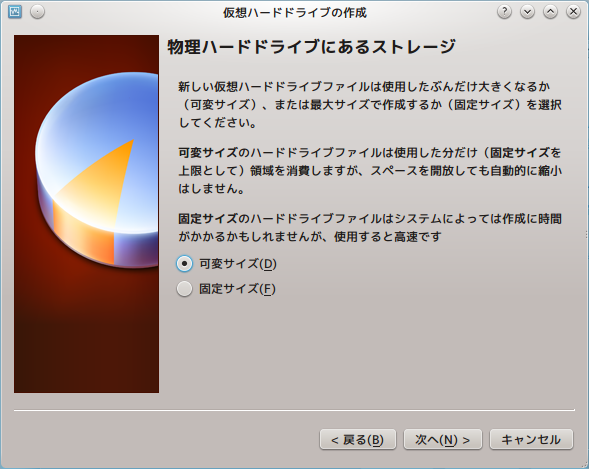
\includegraphics[scale=0.5]{Figs/Fig_VBox/BuildVHD_StorageOnVHD}\protect\caption{仮想ハードディスクの作成(ディスク上のストレージの設定)}
\label{BuildVHD_StorageOnVHD}
\end{figure}


最後に、図\ref{BuildVHD_LocationAndSize}にて仮想ディスクのパスとサイズを設定します。パスは規定のパスで指定される場所以外のところに仮想ディスクを置きたい等の事情が無い限り、デフォルトで構いません。また仮想ディスクのサイズは任意です。構築したい環境にもよりますが、5GB程度もあれば良いでしょう。設定後、「作成」をクリックすると、仮想マシンが仮想ディスクとともに作成されます。VirtualBoxマネージャーが更新され、図\ref{OracleVMVBoxManager_Post}のように、作成した仮想マシンが表示されます。

\begin{figure}[!tbh]
\centering{}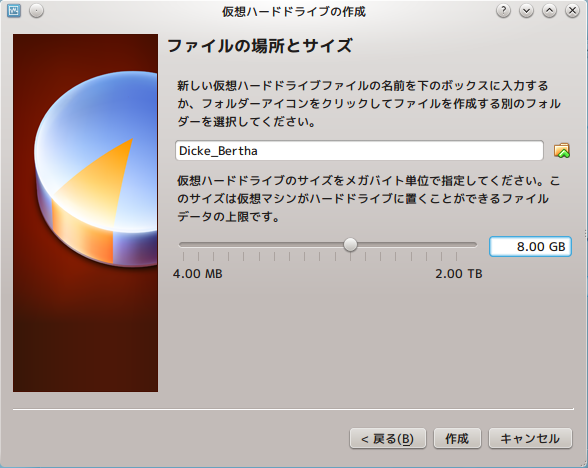
\includegraphics[scale=0.5]{Figs/Fig_VBox/BuildVHD_LocationAndSize}\protect\caption{仮想ハードディスクの作成(ファイルの場所とサイズの設定)}
\label{BuildVHD_LocationAndSize}
\end{figure}


\begin{figure}[!tbh]
\begin{centering}
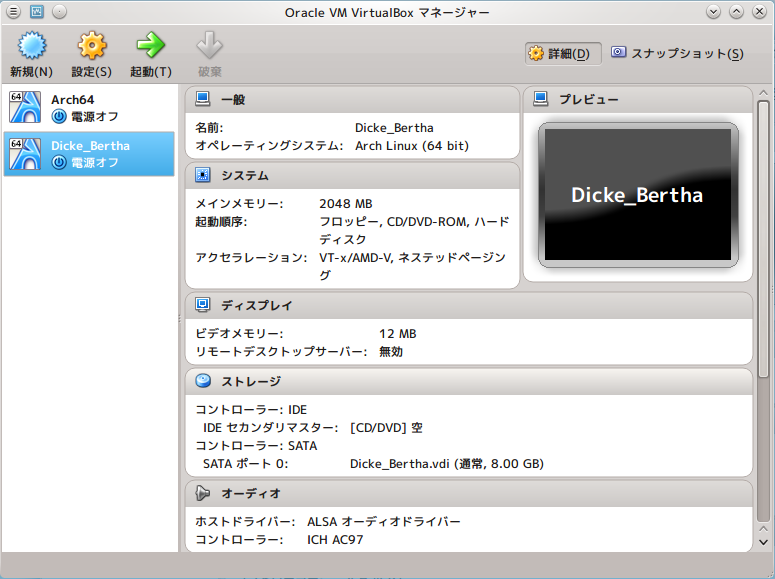
\includegraphics[scale=0.5]{Figs/Fig_VBox/OracleVMVBoxManager2}
\par\end{centering}

\centering{}\protect\caption{仮想マシンの生成完了(Oracle VM VirtualBox マネージャー)}
\label{OracleVMVBoxManager_Post}
\end{figure}



\section{仮想マシンの設定}

前節で仮想マシンの生成が完了したので、次に仮想マシンの設定をしていくことにしましょう。仮想マシンの設定は、図\ref{OracleVMVBoxManager_Post}のVirtualBoxマネージャー上で、設定を編集したい仮想マシンを選択し、「設定」をクリックすることで可能です。「設定」をクリックすると、図\ref{VM_Config}のような設定ウィンドウが開きます。

\begin{figure}[!tbh]
\centering{}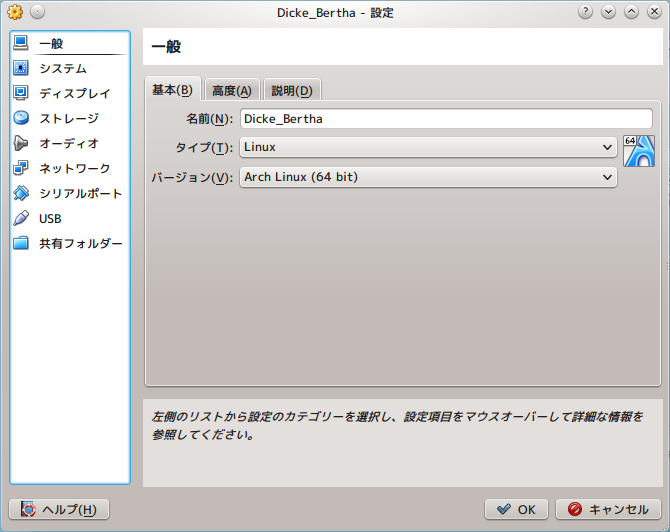
\includegraphics[scale=0.5]{Figs/Fig_VBox/VM_Config}\protect\caption{仮想マシン設定ウィンドウ}
\label{VM_Config}
\end{figure}


このウィンドウを用いて様々な設定が可能ですが、今回は起動デバイスの優先順序を変更するのみに留めたいと思います。OSのインストールを経験したことのある方はわかると思いますが、OSをインストールする場合、コンピュータ内蔵のHDDよりもOSのインストールメディア(DVDドライブやUSBメディアなど)を優先的に起動しないと、OSのインストーラが立ち上がらず内蔵HDDからブートが始まるため、OSをインストールすることができません。

もちろん、起動時の優先順序をこのように変更する必要があるのはOSインストール時だけであり、通常時はHDDをその他のデバイスよりも優先順序を上げておくほうが便利な点が多いことでしょう。

ウィンドウ中の左にあるボックス内の項目から「システム」をクリックし、「マザーボード」タブを選択すると、図\ref{VM_Config_BootPriority}のような状態になります。このうち、「起動順序」の項において、ボックス内のデバイスのうち「CD/DVD-ROM」をクリックし、直右に位置する矢印ボタンで起動順序を最上位に設定します。また、起動時に使用するデバイスは「CD/DVD-ROM」と「ハードディスク」のみですので、各デバイスの左に位置するチェックボックスにチェックが入っていない場合、チェックを入れてください。図\ref{VM_Config_BootPriority}では「フロッピー」にもチェックが入っていますが、フロッピーディスクは今回使用しないので、チェックは任意です。

\begin{figure}[!tbh]
\centering{}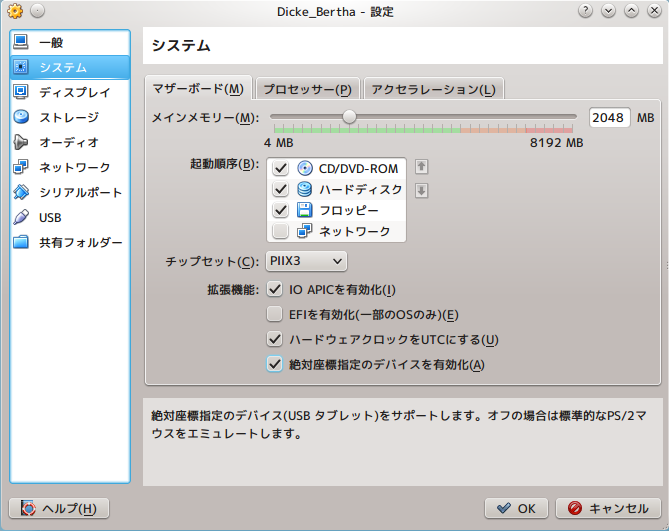
\includegraphics[scale=0.5]{Figs/Fig_VBox/VM_Config_BootPriority}\protect\caption{仮想マシン設定ウィンドウ(「システム」内)}
\label{VM_Config_BootPriority}
\end{figure}



\chapter{仮想マシンの運用}

以上までで作成した仮想マシンを早速運用してみましょう。

今回は、Arch Linuxのインストールイメージを使用し、仮想マシン上へArch Linuxをインストールする、という状況を想定して説明をしていきます。

ここで、Arch Linuxのインストールイメージは何らかの方法で既に物理マシンのディスク上に保存してあるものとします。

まずVirtualBoxを起動し、以上までで作成した仮想マシンを選択して「設定」をクリックし、ウィンドウ中の左にあるボックス内の項目からストレージを選択します(図\ref{VMStorage_Storage})。

\begin{figure}[!tbh]
\centering{}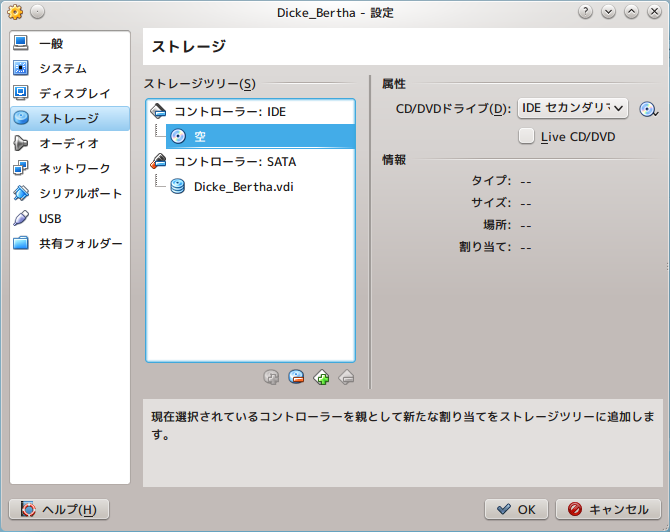
\includegraphics[scale=0.5]{Figs/Fig_VBox/VM_Config_Storage_Setting}\protect\caption{仮想マシン設定ウィンドウ(「ストレージ」内)}
\label{VMStorage_Storage}
\end{figure}


今回設定するのは、「ストレージツリー」中の「コントローラー:IDE」です。図\ref{VMStorage_Storage}のようにCDのアイコンが表示される欄がない場合は、「コントローラー:IDE」を選択し、ストレージツリーのボックス下部にある4種のアイコンのうち、最左のものをクリックし、「CD/DVDデバイスを追加」から「空のディスク」を選択します。続いて、「属性」中のCDのアイコンをクリックし、「仮想CD/DVDディスクファイルの選択」を選び、先ほど保存したArch
Linuxイメージを選択します。

設定し終えたら「OK」をクリックし、設定ウィンドウを閉じます。

VirtualBoxマネージャを確認すると、図\ref{OracleVMVBoxManager_IM}のように、「ストレージ」内のIDEセカンダリマスターに、先程選択したArch
Linuxのイメージファイルが設定されているはずです。

\begin{figure}[!tbh]
\centering{}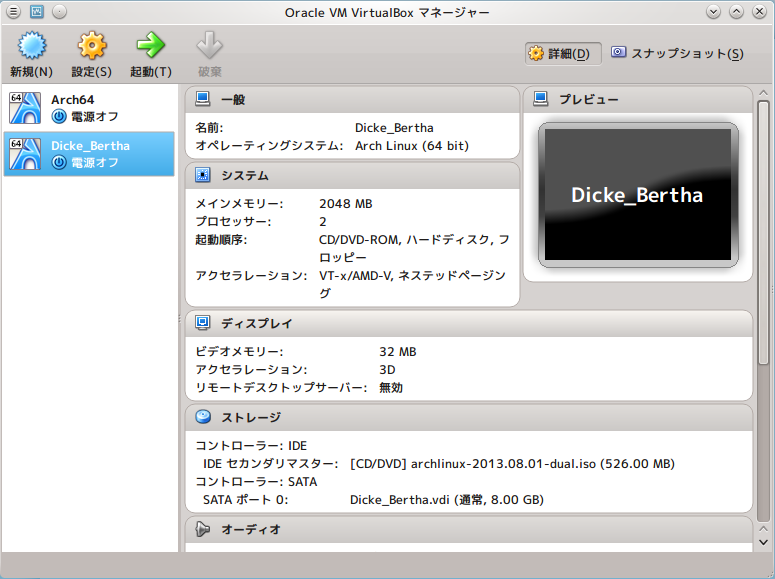
\includegraphics[scale=0.5]{Figs/Fig_VBox/OracleVMVBoxManager3}\protect\caption{インストールイメージの設定結果(Oracle VM VirtualBox マネージャー)}
\label{OracleVMVBoxManager_IM}
\end{figure}


あとは「起動」ボタンをクリックすれば、仮想マシンに電源が投入され、おなじみのブートシーケンスが別のウィンドウ内で開始されます。システムがブートする間、注意事項を記すウィンドウが何度か立ち上がってきますが、内容をよく読んでから「OK」をクリックしてスルーします。何も考えずにスルーしても構わないのですが、たまに仮想マシンにマウスの制御を取り込まれてどうしようもならなくなる時があります。その場合、仮想マシンのウィンドウ右下に表示されているキーを押下するとマウスの制御が実機に復帰します。図\ref{Choose_OS_syslinux}では右Ctrlキーが該当します。何がなんだかわからなくなってパニックにならないように気をつけましょう。

さて、順調に起動処理が進むと、図\ref{Choose_OS_syslinux}のような画面が表示されます。これはブートローダがOSをブートする過程で、起動するOSをユーザが選択するフェーズです。今回仮想マシンにインストールするのは64ビット版のArch
Linuxですので、``Boot Arch Linux (x86\_64)''を選択し、Enterキーを押下します。

\begin{figure}[!tbh]
\centering{}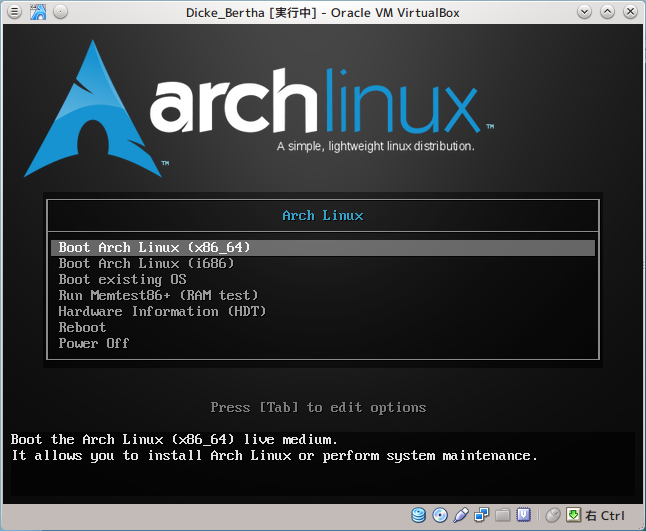
\includegraphics[scale=0.5]{Figs/Fig_ArchLinux/syslinux}\protect\caption{起動するOSを選択する(ブートローダ)}
\label{Choose_OS_syslinux}
\end{figure}


以後のArch Linuxインストールの詳細は、別途「Arch Linuxインストールガイド」をご参照下さい。

OSインストール終了後は、起動デバイスの優先順序を変更するのをお忘れなく。
\end{document}
